% This is based on "sig-alternate.tex" V1.9 April 2009
% This file should be compiled with V2.4 of "sig-alternate.cls" April 2009
%
\documentclass{report}

\usepackage[english]{babel}
\usepackage{graphicx}
\usepackage{tabularx}
\usepackage{subfigure}
\usepackage{enumitem}
\usepackage{url}

\usepackage{color}
\definecolor{orange}{rgb}{1,0.5,0}
\definecolor{lightgray}{rgb}{.9,.9,.9}
\definecolor{java_keyword}{rgb}{0.37, 0.08, 0.25}
\definecolor{java_string}{rgb}{0.06, 0.10, 0.98}
\definecolor{java_comment}{rgb}{0.12, 0.38, 0.18}
\definecolor{java_doc}{rgb}{0.25,0.35,0.75}

% code listings

\usepackage{listings}
\lstloadlanguages{Java}
\lstset{
	language=Java,
	basicstyle=\scriptsize\ttfamily,
	backgroundcolor=\color{lightgray},
	keywordstyle=\color{java_keyword}\bfseries,
	stringstyle=\color{java_string},
	commentstyle=\color{java_comment},
	morecomment=[s][\color{java_doc}]{/**}{*/},
	tabsize=2,
	showtabs=false,
	extendedchars=true,
	showstringspaces=false,
	showspaces=false,
	breaklines=true,
	numbers=left,
	numberstyle=\tiny,
	numbersep=6pt,
	xleftmargin=3pt,
	xrightmargin=3pt,
	framexleftmargin=3pt,
	framexrightmargin=3pt,
	captionpos=b
}

% Disable single lines at the start of a paragraph (Schusterjungen)

\clubpenalty = 10000

% Disable single lines at the end of a paragraph (Hurenkinder)

\widowpenalty = 10000
\displaywidowpenalty = 10000
 
% allows for colored, easy-to-find todos

\newcommand{\todo}[1]{\textsf{\textbf{\textcolor{orange}{[[#1]]}}}}

% consistent references: use these instead of \label and \ref

\newcommand{\lsec}[1]{\label{sec:#1}}
\newcommand{\lssec}[1]{\label{ssec:#1}}
\newcommand{\lfig}[1]{\label{fig:#1}}
\newcommand{\ltab}[1]{\label{tab:#1}}
\newcommand{\rsec}[1]{Section~\ref{sec:#1}}
\newcommand{\rssec}[1]{Section~\ref{ssec:#1}}
\newcommand{\rfig}[1]{Figure~\ref{fig:#1}}
\newcommand{\rtab}[1]{Table~\ref{tab:#1}}
\newcommand{\rlst}[1]{Listing~\ref{#1}}

% General information

\title{Distributed Systems -- Assignment 2}

% Use the \alignauthor commands to handle the names
% and affiliations for an 'aesthetic maximum' of six authors.

\numberofauthors{3} %  in this sample file, there are a *total*
% of EIGHT authors. SIX appear on the 'first-page' (for formatting
% reasons) and the remaining two appear in the \additionalauthors section.
%
\author{
% You can go ahead and credit any number of authors here,
% e.g. one 'row of three' or two rows (consisting of one row of three
% and a second row of one, two or three).
%
% The command \alignauthor (no curly braces needed) should
% precede each author name, affiliation/snail-mail address and
% e-mail address. Additionally, tag each line of
% affiliation/address with \affaddr, and tag the
% e-mail address with \email.
%
% 1st. author
\alignauthor Robin Guldener\\
	\affaddr{ETH ID 11-930-369}\\
	\email{robing@student.ethz.ch}
% 2nd. author
\alignauthor Nico Previtali\\
	\affaddr{ETH ID 11-926-433}\\
	\email{pnico@student.ethz.ch}
%% 3rd. author
\alignauthor Lukas Bischofberger\\
	\affaddr{ETH ID 11-915-907}\\
	\email{lukasbi@student.ethz.ch}
}
%\and  % use '\and' if you need 'another row' of author names
%% 4th. author
%\alignauthor Student Four\\
% 	\affaddr{ETH ID XX-XXX-XXX}\\
% 	\email{four@student.ethz.ch}
%% 5th. author
%\alignauthor Student Five\\
% 	\affaddr{ETH ID XX-XXX-XXX}\\
% 	\email{five@student.ethz.ch}
%% 6th. author
%\alignauthor Student Six\\
% 	\affaddr{ETH ID XX-XXX-XXX}\\
% 	\email{six@student.ethz.ch}
%}


\begin{document}

\maketitle

\begin{abstract}
For the implementation of this assignment we made use of the two lab provided HTC desire number 25 and 37. We were able to implement all the assigments listed on the assignment sheet and to our best knowledge all services are working flawlessly. Our enhancements include the graphing of temperatures using the Google REST Charts API as well as [WHATEVER YOU ENHANCED THE SERVER WITH].
\end{abstract}

\section{Introduction}

Web Services allow for the easy inclusion of services provided by any entity over the internet. One of the main advantages of web services are that they allow for a simple implementation of the service oriented architecture as they abstract and implement many of the common networking problems encountered in implementing such an architecture. Additionally web services have the advantage of making it dead simple to include functionality implemented by 3rd parties by simply calling their services with the required parameters.

RESTful Web Services use the HTTP verbs to specify the action to perform on an object identified by the service URL. The key advantage of this method over WS\hbox{-}* Web Services is their simplicity due to the implicit encoding of the action in the HTTP verb. However as the same time this is also one of their main drawbacks as they are somewhat more limited in terms of functionality and extensibility than WS\hbox{-}* Web Services.

WS\hbox{-}* Web Services describes a class of Web Services which make use of the WSDL protocol to advertise their capabilities to other services and usually implement the SOAP protocol for actual requests to the service (however, this is not a requirement, WSDL allows for any arbitrary request protocol to be specified). Their main advantage is the wide range of configuration and extensibility options as well as the automated service discovery. This flexibility comes with a price though and thus usually WS\hbox{-}* services are usually considerably more complex than their REST equivalents.

\section{RESTful Web Services}
%\begin{itemize}
%	\item Describe shortly, how you designed your application to implement this Task. Which Android core elements did you use (e.g., Activity, Service, AsyncTask, Intent)?
%	\item Explain why it is beneficial (or even required, since Android 3.0), to off-load networking tasks to AsyncTask. \textbf{Hint:} Explain what \emph{blocking}-methods are in the context of handling I/O Streams.
%	\item Explain how you make use of the different methods provided by AsyncTask, such as \texttt{doInBackground}, \texttt{onPreExecute}, \texttt{onProgressUpdate}, \texttt{publishProgress} or \texttt{onPostExecute}.
%\end{itemize}
In this assignment we retrieve the temperature of Spot 1 \cite{temperatureSpot1}, which is obviously served by a RESTful Web Service. The application consists of a single Main Activity. This Activity provides four buttons to invoke the RESTful Web Service. The first and second button will make HTTP requests using different libraries. The third and fourth button will make use of the  \texttt{content negotitation} mechanism. The last button displays a visualization using cloud services explained in-depth in section Cloud Services. All HTTP requests are invoked asynchronous, handled by the Main Activity, using the AsyncTask class.

Since Android 3.0 attempts to perform a networking operation must not be handled on the GUI thread which is simultaneously the main thread of the application. This makes perfect sense because network operations include blocking methods. Blocking methods are those method which block the executing thread until the operation finished. Famous example of blocking method is InputStream \texttt{read()} method which blocks until all data from InputStream has been read completely. Networking operations in Java use a lot of InputStreams. Therefore it is necesserary to handle networking operations in a seperate thread to avoid blocking the main thread. If the main thread would be blocked, user input can not be made. For this reason Android provides an \texttt{AsyncTask} class.

\lstset{language=Java,caption={Using AsyncTask},label=asynctask} 
	\begin{lstlisting}
// Our worker which performs networking operations
private class RESTWorker extends AsyncTask<String, Void, String> {
	...
}
	\end{lstlisting}

The AysncTask class serves several important methods, such as \texttt{doInBackground}, \texttt{onPostExecute}. \texttt{doInBackground} performs all operations asynchronous in background on a seperate thread. We use this method to do all the networking operations such as sending HTTP GET requests. Full advantage shows us AsyncTask when it happens to update UI elements. For this reason, AsynTask provides a method \texttt{onPostExecute} which is synchronized to the main thread (rember, this is also the UI thread). Therefore one can easily update UI elements without having to worry about the synchronization.

\lstset{language=Java,caption={Updating UI elements},label=uielements} 
	\begin{lstlisting}
	@Override
		protected void onPostExecute(String result) {
			super.onPostExecute(result);
			// this method is synchronized with the user main thread (handled by Android), so no problems occur...
			if (result != null) {
				switch (mode) {
					default:
						// clear chart and write REST response
						imgChart.setImageResource(R.drawable.blank);
						if (retrieveWithLabelAndWrite) writeResult(result);
						break;
					case RESTWorker.MODE_CHART:
						// clear REST response and display chart
						writeResult("");
						imgChart.setImageBitmap(bmp);
						break;
				}
			}
		}
	\end{lstlisting}

\begin{figure}
    \centering
    \subfigure[Extracted value from JSON repsonse]{
        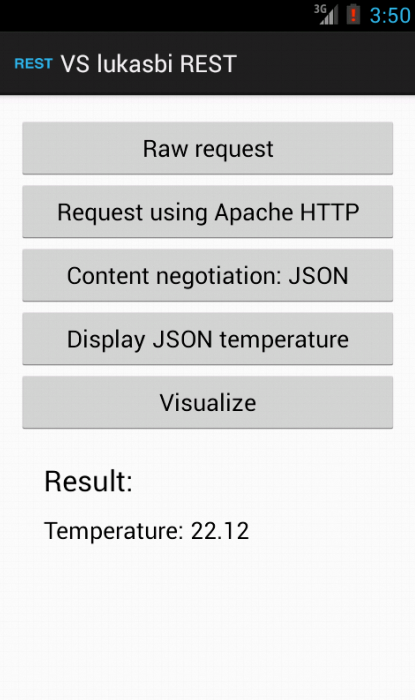
\includegraphics[height=4.2cm]{rest-1.png}
        \lfig{axis}   
    }
    \subfigure[Raw JSON response]{
        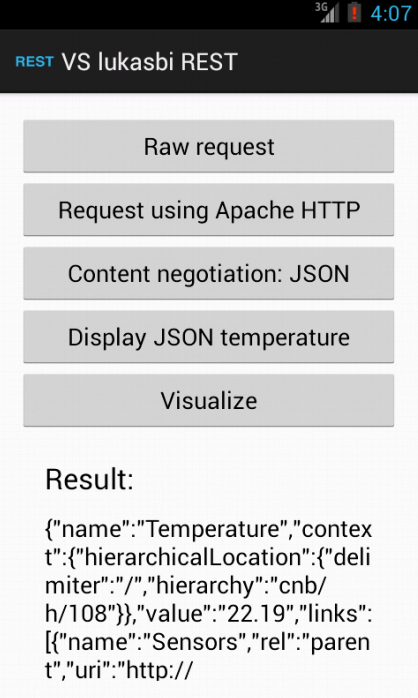
\includegraphics[height=4.2cm]{rest-2.png}
        \lfig{axis}   
    }
    \subfigure[Raw HTML response]{
        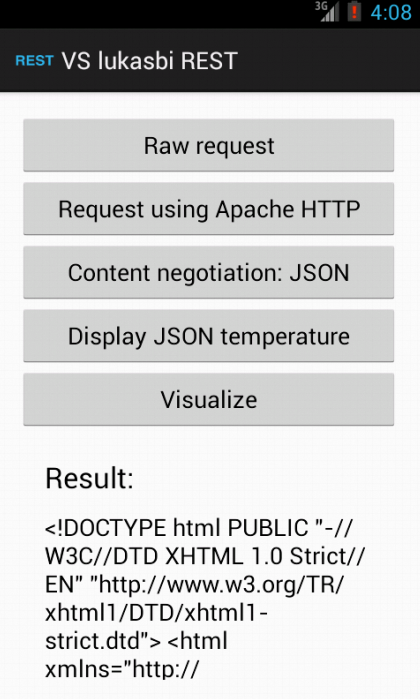
\includegraphics[height=4.2cm]{rest-3.png}
        \lfig{axis}   
    }
    \caption{GUI of Main Activity showing different responses}
\end{figure}

\section{WS-* Web Services}
As a first task for the WS-* web services part we had to think about how we would implement invoking a WS-* web service only using the \texttt{java.net} library. The following steps would have to be pursued:
\begin{enumerate}
	\item Get the web service's description by obtaining its WSDL file from a predefined address. This could be downloaded with an HTTP GET request utilizing the \texttt{URLConnection} class like thus:
	\lstset{language=Java,caption={Getting data from a webserver using HTTP GET},label=httpget} 
	\begin{lstlisting}
// Assuming url is a String holding the url for the WSDL
URLConnection connection = new URL(url).openConnection();
InputStream stream = connection.getInputStream();
	\end{lstlisting}
	\item Read the entire response from the input stream and parse the response using an XML library (or write your own). From the WSDL extract the URL of the web service you wish to call by looking at the \texttt{PortType} section and finding the \texttt{operation} which you would like to perform. Also be sure to check the appropriate input and output configuration as well as the actual transport protocol (usually SOAP) for your \texttt{operation} from the \texttt{binding} section
	\item Prepare the actual request, here we will use SOAP. For SOAP this means creating the request XML by defining the SOAP envelope and specifying the header and body information required by the \texttt{operation} that is to be queried/called. In this example we a re calling one of the web services provided by the VSLAB and request a list of all discovered SunSPOTs:
	\lstset{language=XML,caption={SOAP Request},label=httpget} 
	\begin{lstlisting}
<?xml version="1.0" encoding="UTF-8"?><S:Envelope xmlns:S="http://schemas.xmlsoap.org/soap/envelope/">
    <S:Header/>
    <S:Body>
        <ns2:getDiscoveredSpots xmlns:ns2="http://webservices.vslecture.vs.inf.ethz.ch/"/>
    </S:Body>
</S:Envelope>
	\end{lstlisting}
	\item Now that the request is ready it has to be actually transferred to the endpoint. For this we establish a new \texttt{URLConnection} with the endpoint and send our SOAP request using the HTTP POST keyword to the endpoint like this:
	\lstset{language=Java,caption={POST-ing a SOAP request to the endpoint},label=httpget} 
	\begin{lstlisting}
// Assuming url is a String holding the url for the web service endpoint & soap is the SOAP XML request string
URLConnection connection = new URL(url).openConnection();
connection.setDoOutput(true); // Triggers POST.
connection.setRequestProperty("Content-Type", "application/xml+soap;charset=" + charset);
OutputStream output = connection.getOutputStream();
try {
     output.write(soap.getBytes(charset));
} finally {
     try { output.close(); } catch (IOException logOrIgnore) {}
}
InputStream response = connection.getInputStream();
	\end{lstlisting}
	\item Finally we parse the XML from the response to obtain the data we asked for. Done!
\end{enumerate}


For the second part of the WS\hbox{-}* Web Services we implemented a simple Android application that downloads the latest temperature from Spot3 using SOAP requests. Our application consists of only two classes, one subclass of Activity, which implements our MainActivity, and one subclass of AsyncTask, which perfoms all the required networking in the background. This second class was largely recycled from Task 1 and adapted to fit the use of the WS\hbox{-}* Web Services.

To be able to perform requests against a Web Service one must first know which services and actions exist. This part is covered by WSDL files and we retrieved the WSDL file corresponding to the Web Service for this task from the lecture website. From the WSDL we were able to determine the service endpoint as well as the action name and the parameters to pass in. With this information we were able to actually build the requests required, in this case SOAP requests. The actual creation of the SOAP request is performed by the ksoap2-androidlibrary\cite{ksoap2} which takes care of forming the appropriate XML strings.

The main advantage of SOAP using XML instead of a binary format is that it is completely platform independent and allows for the encoding of arbitrary objects. The process of transforming these objects back into platform specific objects (ie. Java objects if the final destination platform is Java) is commonly referred to as unmarshalling.

\section{Cloud Services}
%\begin{itemize}
%	\item Which diagram type did you choose? You can show a screen shot and describe your custom functionalities, if you have implemented any.
%\end{itemize}
The measured temperatures of Spot 1 are visualized with a bar chart. The chart is generated by sending a HTTP POST request to the Google Chart Tools Image cloud service \cite{googleChart}. The difficulty was to scale the data so that they correspond to the axes.

\begin{figure}
    \centering
    \subfigure {
        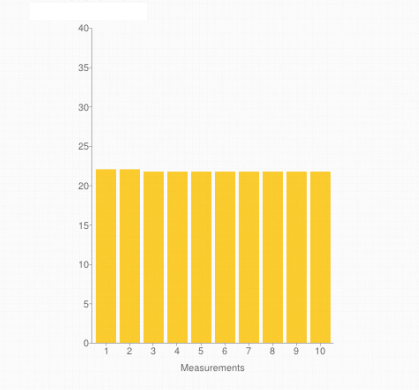
\includegraphics[height=4.2cm]{rest-5.png}
        \lfig{axis}   
    }
    \caption{Temperature chart}
\end{figure}


\section{Your Phone As a Server}
\begin{itemize}
	\item The implementation of the server relies on an Activity to start and stop the server and some background threads to handle network action and multitasking. 
	%\item Describe shortly, how you designed your application to implement this Task. Which Android core elements did you use this time?
	\item Java code for accepting multiple connections. Each time the socket is bound to an incoming connection it gets assigned to a helper thread which computes the response. The socket is then free again for a new connection.
		\begin{lstlisting}
while(!Thread.currentThread().isInterrupted()) {
	try {
		socket = serverSocket.accept();	
							
		//start a new thread to handle connection
		ServerHelperThread sth = new ServerHelperThread(socket, mContext);
		new Thread(sth).start();
	} catch (IOException e) {
		e.printStackTrace();
	}
}	
		\end{lstlisting}
	%\item Show in a control flow diagram, pseudo code or your actual Java implementation, how you (would) do the handling of the connections on the server side. If you weren't able to implement the multi threading, explain it for a single threaded version.
	\item We implemented both sensing and actuation. For the sensing there is the possibility to see the list of the sensors and also to see the details of a chosen specific sensor. \\
	Actuation was implemented for vibrating the phone for a specified amount of time (by the slider) and for starting some kind of music on the phone. \\
	We implemented both sensing and actuation by the GET method. The GET method is easier to implement and the data is easier to acquire. Secondly we didn't manage to safely get the data of the POST method, apparently the browser didn't send an end of the header and the InputStreamReader was waiting for more data, so we stuck with the GET method.
	%\item Did you implement sensing and/or actuation? How did you make use of the different HTTP methods, e.g. GET or PUT?
\end{itemize}

\section{Enhancements}

This is usually the final part of an assignment.
Here you are free to describe what you did, however, stick to a concise, scientific writing style.

\section{Conclusion}

%Give an overall conclusion that summarizes the main challenges you encountered and your lessons learned.
One conclusion that we obtained is dealing with RESTful Web Services is much easier und comfortable than with WS-* Web Services.

% The following two commands are all you need in the
% initial runs of your .tex file to
% produce the bibliography for the citations in your paper.
\bibliographystyle{abbrv}
\bibliography{report}  % sigproc.bib is the name of the Bibliography in this case
% You must have a proper ".bib" file

%\balancecolumns % GM June 2007

\end{document}
